% This is a basic Math Paper

\documentclass[11pt]{article}

% Preamble

\usepackage[margin=1in]{geometry}
\usepackage{amsfonts, amsmath, amssymb}
\usepackage{gensymb}
\usepackage{fancyhdr, float, graphicx}
\usepackage[utf8]{inputenc} % Required for inputting international characters
\usepackage[T1]{fontenc} % Output font encoding for international characters
\usepackage{fouriernc} % Use the New Century Schoolbook font
\usepackage[nottoc, notlot, notlof]{tocbibind}


% Header and Footer
\pagestyle{fancy}
\fancyhead{}
\fancyfoot{}
\fancyhead[L]{\textit{\Large{Engineering Mechanics Experiment 9}}}
%\fancyhead[R]{\textit{something}}
\fancyfoot[C]{\thepage}
\renewcommand{\footrulewidth}{1pt}



% Other Doc Editing
% \parindent 0ex
%\renewcommand{\baselinestretch}{1.5}

\begin{document}
	
	\begin{titlepage} 
		\centering 
		
		%---------------------------NAMES-------------------------------
		
		\huge\textsc{
			MIT World Peace University
		}\\
	
		\vspace{0.75\baselineskip} % space after Uni Name
		
		\LARGE{
			Engineering Mechanics\\
			First Year B. Tech, Trimester 1
		}
	
		
		\vfill % space after Sub Name
		
		%--------------------------TITLE-------------------------------
		
		\rule{\textwidth}{1.6pt}\vspace*{-\baselineskip}\vspace*{2pt}
		\rule{\textwidth}{0.6pt}
		\vspace{0.75\baselineskip} % Whitespace above the title
		
		
		
		\huge{\textsc{
				Graphical Solution to find Reactions of Beams under the influence of a Co-Planar Non-Concurrent Force System
			}} \\
		
		
		
		\vspace{0.5\baselineskip} % Whitespace below the title
		\rule{\textwidth}{0.6pt}\vspace*{-\baselineskip}\vspace*{2.8pt}
		\rule{\textwidth}{1.6pt}
		
		\vspace{1\baselineskip} % Whitespace after the title block

		%--------------------------SUBTITLE --------------------------	
			
		\LARGE\textsc{
			Experiment 9\\
			Practical Report
		} % Subtitle or further description
		\vfill
		
		%--------------------------AUTHOR-------------------------------
		
		Prepared By
		\vspace{0.5\baselineskip} % Whitespace before the editors
		
		\Large{
			Krishnaraj Thadesar \\
			Division 9, Roll No. 54
		}
		
		
		\vspace{0.5\baselineskip} % Whitespace below the editor list
		\today

	\end{titlepage}
	
	
\tableofcontents
\thispagestyle{empty}
\clearpage


\setcounter{page}{1}

\section{Objective}
To find Graphically and Analytically the resultant of a set of problems involving Non-Concurrent Co-Planar Force System, and to compare the results thereby finding the Percentage Error.

\section{Theory}
The Following laws and concepts have been used in this experiment.

\subsection{Force law of equilibrium}
\textit{When all the forces that act upon an object are balanced, then the object is said to be in a state of equilibrium. The forces are considered to be balanced if the rightward forces are balanced by the leftward forces and the upward forces are balanced by the downward forces. This however does not necessarily mean that all the forces are equal to each other.}

\subsection{Moment of a Force}

The Moment of a force is a measure of its tendency to cause a body to rotate about a specific point or axis. This is different from the tendency for a body to move, or translate, in the direction of the force. \\

In order for a moment to develop, the force must act upon the body in such a manner that the body would begin to twist. This occurs every time a force is applied so that it does not pass through the centroid of the body.
Moment $ \tau $ can be defined as
$$\tau=F\ \mathrm{x}\ r$$

\subsection{Equilibrium and Rigid Body in Equlibrium}

Knowledge of the forces required to maintain an object in equilibrium is essential in understanding the nature of bodies at rest and in motion. To determine if a body is in equilibrium, the overall effect of all the forces acting on it must be assessed. All the forces that act on an object result in essentially one force that influences the object's motion. The force which results from all the forces acting on a body is defined as the net force.\\
Since an object in equilibrium is considered to be in a state of balance, it can be summarised that the net force on the object is equal to zero. That is, if the vector sum of all the forces acting on an object is equal to zero, then the object is in equilibrium. 
The first condition of equilibrium, a consequence of Newton's first law, may be written in vector form, "A body will be in translational equilibrium if and only if the vector sum of forces exerted on a body by the environment equals zero."
For example, if three forces act on a body it is necessary for the following to be true for the body to be in equilibrium.
$$F1 + F2 + F3 = 0\	\mathrm{or}\	\Sigma_F = 0 $$
This condition applies to objects in motion with constant velocity and to bodies at rest or in static equilibrium.\\

\textit{A rigid body is in equilibrium when it is not undergoing a change in rotational or translational motion. This equilibrium requires that two conditions must be met. The forces acting on it must add up to zero, and the moments must also add up to zero. It can be represented as:}
$$ \Sigma_F=0\  \mathrm{and}\  \Sigma_M=0 $$
\subsection{Beams}
Beam is a horizontal member used to carry vertical load, shear load and sometime horizontal load. It is the major component of building structures. It mainly used in construction of bridges, trusses, and other structures which carry vertical load.

\subsection{Space and Polar Diagrams}
\subsubsection{Space Diagram}
A drawing of a structure that indicates its form as well as means of its support and loading conditions.
\subsubsection{Polar Diagram}
In case of non-concurrent or parallel force system the point of
application of resultant can be found out by constructing polar diagram. Polar
diagram is obtained from the vector diagram. To construct a polar diagram, any
point “O” known as pole is chosen near the vector diagram and the points on the
vector diagram are joined to it. The lines joined in this way are known as rays. 
\subsection{Funicular Polygon}

a graphical method of finding the reactive forces and resultants of a system of forces, constructing bending-moment diagrams, determining the rational shapes of arched and suspended systems, and solving other problems of the statics of two-dimensional systems.\\

The construction of funicular polygons is based on the conception of a polygon formed by an axis that is fixed at the ends of a weightless thread (string), which is tensioned by the forces acting on it. The construction of a funicular polygon together with a force polygon (see Figure) is also used to determine the geometric characteristics of planar cross sections and to solve certain problems in engineering hydraulics, economics, and other fields.
\begin{figure}[H]
	\centering
	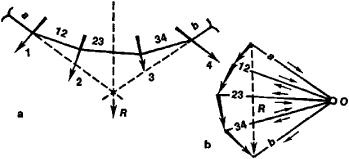
\includegraphics[scale=0.5]{fp.jpg}
	\label{fig: Polygon Law}

\end{figure}

\subsection{Coplanar and non-concurrent force system}
These forces do not meet at a common point; however, they lie in a single plane, for example, forces acting on a beam as shown in Figure. 

\begin{figure}[H]
	\centering
	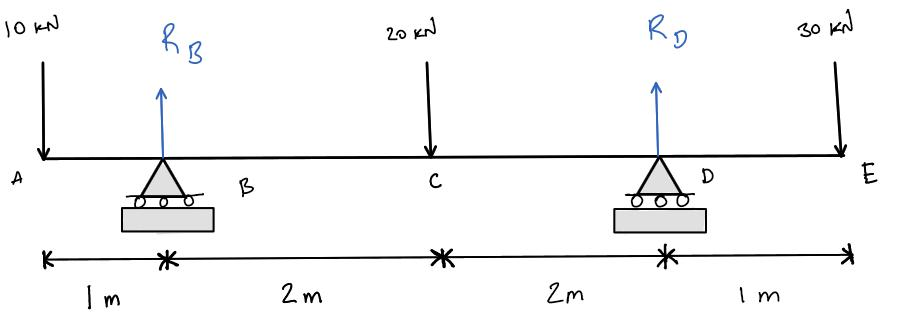
\includegraphics[scale=0.3]{ncfc.jpg}
	\label{fig: Polygon Law}
\end{figure}

\section{Procedure}
In non-concurrent force system, the following procedure is adopted to find resultant: 
\begin{enumerate}
	\item Draw space diagram to suitable scale as discussed for concurrent force system.
	\item Draw vector diagram as discussed for concurrent force system.
	\item Select a convenient point in the vector diagram called the pole 'o'. From this pole, draw rays $o a, o b, o c \ldots$ etc. to points $a, b, c, \ldots$ etc. of the vector diagram. This diagram is called the polar diagram.
	\item Draw lines parallel to the rays in polar diagram by maintaining their order in the respective spaces of space diagram. The first line oa is to be drawn in space $A$. The next line parallel to $o b$ is drawn from the point of intersection of the first line with the first force. Each subsequent line is drawn form the point of intersection of previous line with its corresponding force. This diagram is known as funicular polygon or link polygon.
	\item Resultant is obtained by finding magnitude and direction from vector diagram. Its point of application is obtained by extending the first and last lines of funicular polygon to locate their point of intersection. From this point, a line is drawn parallel to the resultant obtained in vector diagram. The point where this line intersects the given object is the point of application of the resultant.
	\item If the object is in equilibrium, then the vector diagram and the funicular polygon must be closed figures. This concept is used to find reactions in beams. The procedure discussed above is illustrated in subsequent problem.
\end{enumerate}
\subsection{Problem 1}
\begin{enumerate}
	\item Draw the given beam $\mathrm{ABCD}$ to scale as shown in Fig. Represent the spaces according to Bow's notation as (A), B), (C) (D) and (E).
	\item Draw vector diagram. As all the forces are vertical all the vectors and their resultant will be in one line. In Figure, a scale of $1 \mathrm{~cm} \equiv 5 \mathrm{kN}$ is chosen. Choose any point $a$ in the plane. So, $a b=2 \mathrm{~cm} \equiv 10 \mathrm{kN}$ represents the force at $A$. From $b$, a downward line $b c$ of $3 \mathrm{~cm}$ is drawn representing $15 \mathrm{kN}$ force. From $C$, upword line $c d=2 \mathrm{~cm}$ representing $10 \mathrm{kN}$ force at $C$ and from $d$, upward line of $d e=4 \mathrm{~cm}$ representing $20 \mathrm{kN}$ force at $D$ are drawn. ae represents resultant force in magnitude and direction. By measurement,
	$$
	a e=5 \mathrm{~cm}
	$$
	Converting to scale,
	$$
	\begin{aligned}
		&R=5 \times 5 \\
		&R=25 \mathrm{kN} \uparrow
	\end{aligned}
	$$
	\item Choose an arbitrary point $o$ the pole and draw rays $o a, o b, \ldots$ etc. to form the polar diagram.
	\item Draw line $o a$ in space diagram parallel to ray oa in polar diagram. From the point of intersection of this line with line of action of $10 \mathrm{kN}$ force at $A$, draw line ob parallel to $o b$. Similarly draw $o c, o d$, and $o e$.
	\item Extend oa and oe and from the point of their intersection draw a line parallel to $a e$ in polar diagram which represents the resultant $R$. The point of intersection of $R$ with the beam $A D$ gives point of application. By measurement,
	$$
	x=9.1 \mathrm{~cm}
	$$
	Converting to scale,
	$$
	\begin{aligned}
		x &=9.1 \times 0.5=4.55 \mathrm{~m} \\
		x &=4.55 \mathrm{~m} \text { form } \mathrm{A}
	\end{aligned}
	$$
	By analytical calculation, $R=25 \mathrm{kN} \uparrow$ and $x=4.6 \mathrm{~m}$ from $A$.
	
\end{enumerate}
\subsection{Problem 2}
\begin{enumerate}
	\item Draw the space diagram by drawing the beam to scale and naming the spaces between only the loads as $A$, B , (C), and D as shown in Fig.
	\item Draw vector diagram for the loads, choose a pole and draw rays to complete the polar diagram.
	\item Draw a line parallel to the first ray on in space diagram starting from any point on line of action of $R_{B}$ and intersecting line of action of $10 \mathrm{kN}$ force acting at $A$. From point of intersection of oa with line of action of $10 \mathrm{kN}$, draw line parallel to ob to intersect line of action of $20 \mathrm{kN}$ at $C$. From this point of intersection, draw line parallel to $o c$ to intersect line of action of $30 \mathrm{kN}$ force acting at $E$. From this point of intersection, draw line parallel to od to intersect line of action of $R_{D}$. Draw line from this point of intersection to the point of intersection of on $\mathrm{K}$. $R_{B}$. This is the closing line for funicular polygon.
	\item Draw ray from pole in polar diagram parallel to the closing line for funicular polygon to intersect the line ad at point $p$.
\end{enumerate}
	
\subsection{Problem 3}
\begin{enumerate}
	\item Draw the space diagram by drawing the beam to scale and naming the spaces between the loads as $A, B$, and (C) as shown in Fig.
	\item Draw vector diagram for the loads, choose a pole and draw rays to complete the polar diagram.
	\item When there is hinge, always start from the hinge. Draw line parallel to ray $o c$ form $D$ in space diagram to intersect line of action of $15 \mathrm{kN}$ force acting at $C$. From this point of intersection, draw line parallel to ray ob to intersect line of action of $10 \mathrm{kN}$ force acting at $B$. From this point of intersection, draw line parallel to on to intersect line of action of $R_{A} .$ Draw closing line of funicular polygon from $D$ to this point of intersection.
	\item Draw ray parallel to closing line in polar diagram. Draw a line parallel to $R_{A}$ which is at $60^{\circ} \simeq$ form point $a$. Let $P$ be the point of intersection of these lines then $p a$ represents $R_{A}$ and $c p$ represents $R_{D} .$ By measurement,
	$$
	p a=3 \mathrm{~cm} \text { and } c p=2.9 \mathrm{~cm}
	$$
\end{enumerate}


\pagebreak
\section{Analytical Method}


Q1. Determine the magnitude, direction and point of application of resultant from A for the force system shown in Fig. which acts on beam AD.
\begin{figure}[H]
	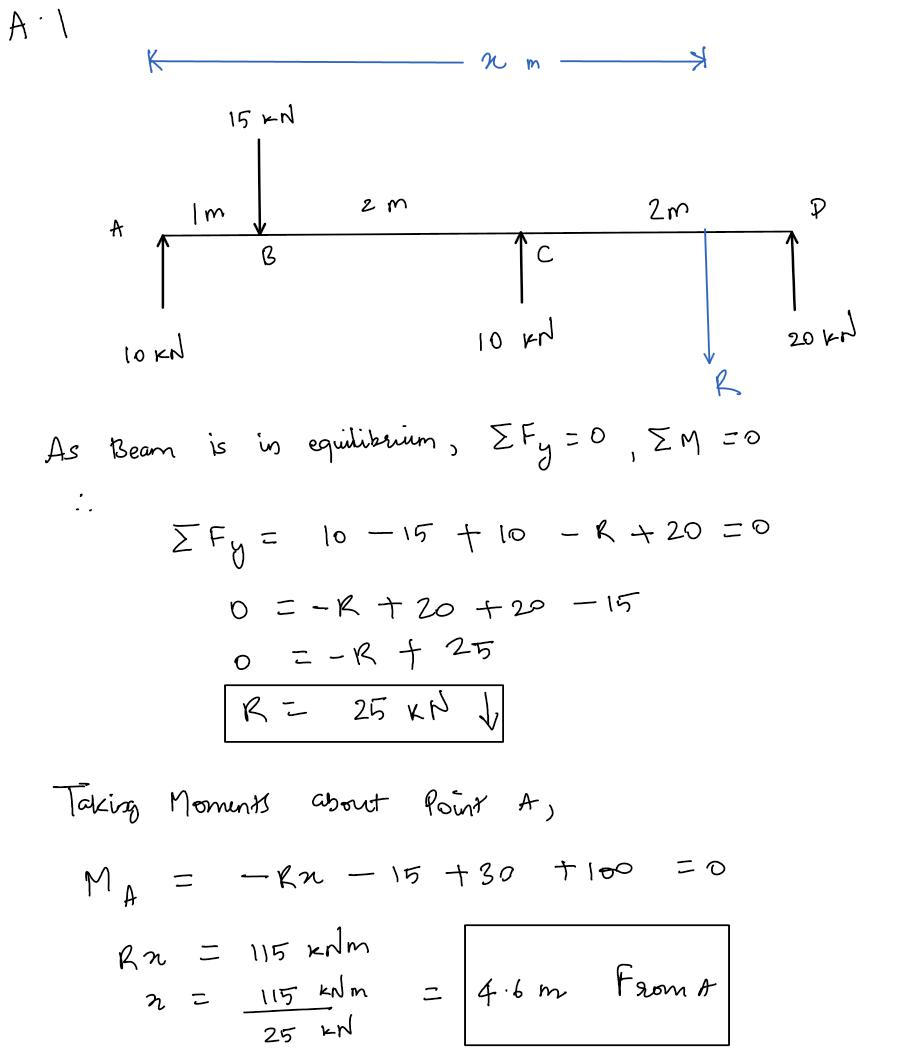
\includegraphics[scale=0.5]{a1.jpg}
	\label{fig: Polygon Law}
\end{figure}


\pagebreak
Q2. Determine the beat reactions for the beam shown in the figure. 
\begin{figure}[H]
	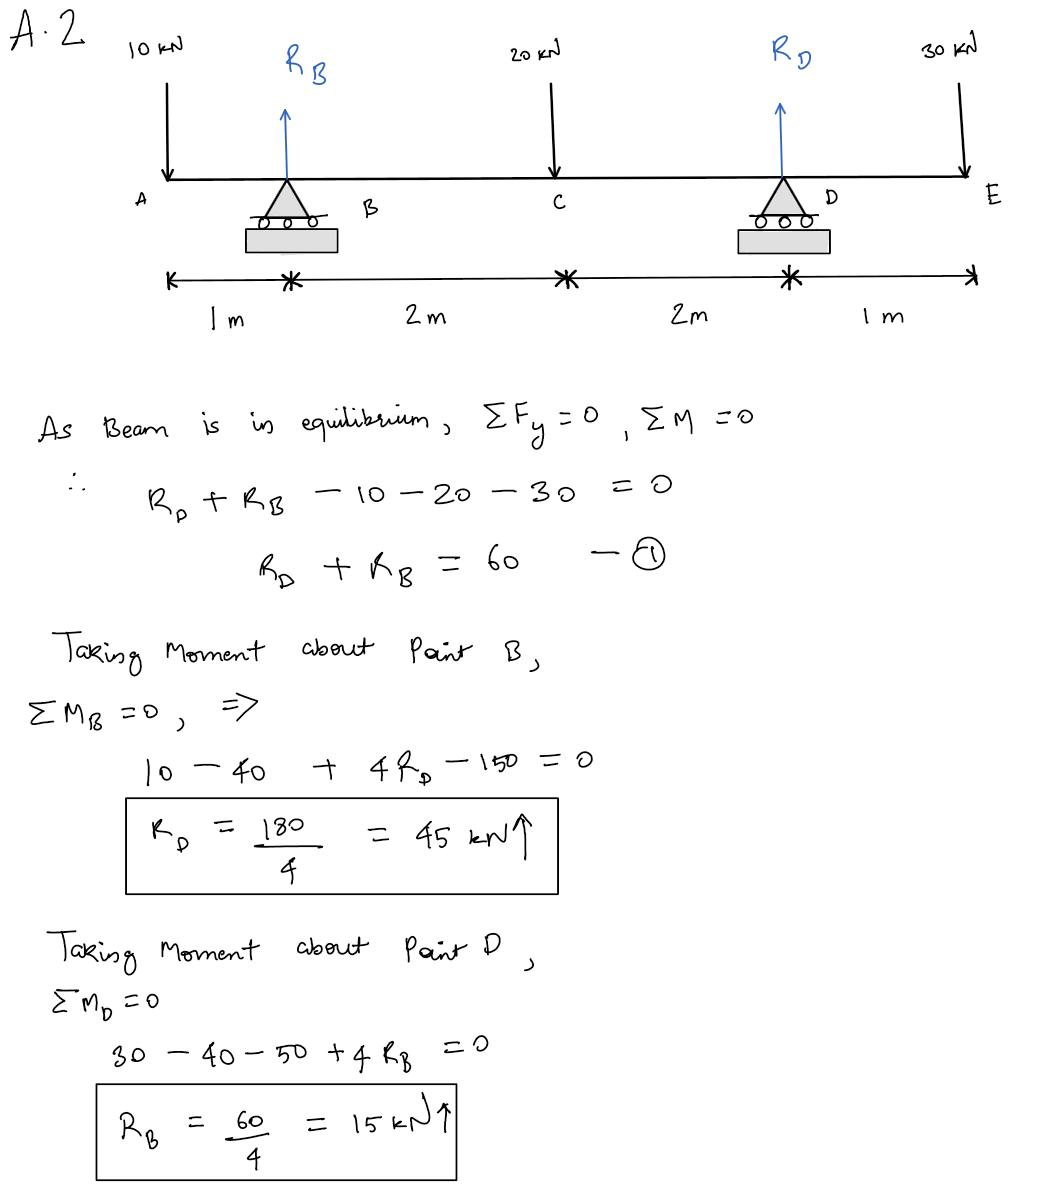
\includegraphics[scale=0.45]{a2.jpg}
	\label{fig: Polygon Law}
\end{figure}
\pagebreak

Q3. Determine support reactions for the beam loaded and supported as shown in the figure.
\begin{figure}[H]
	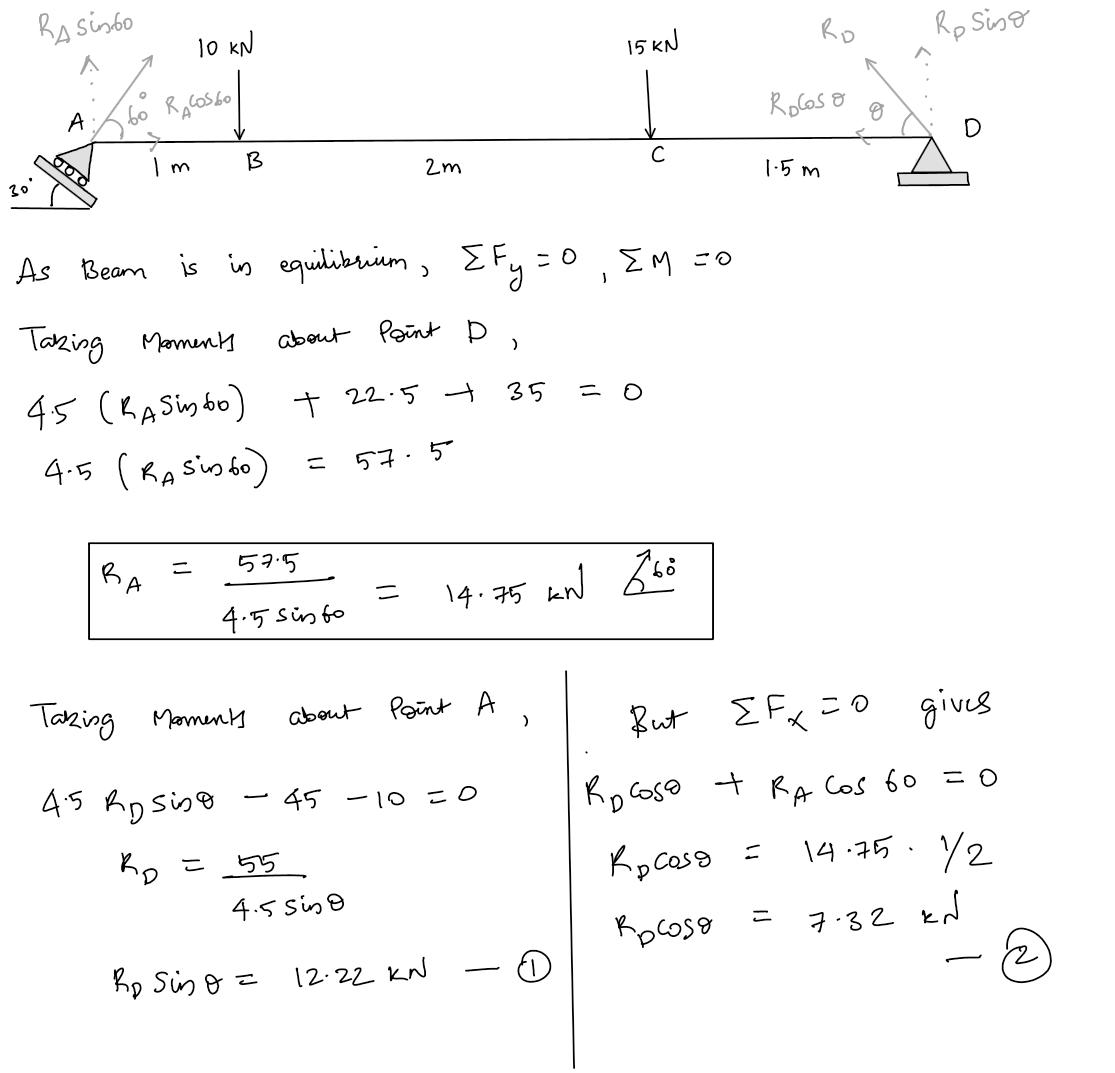
\includegraphics[scale=0.5]{a31.jpg}
	\label{fig: Polygon Law}
\end{figure}

\pagebreak
\begin{figure}[H]
	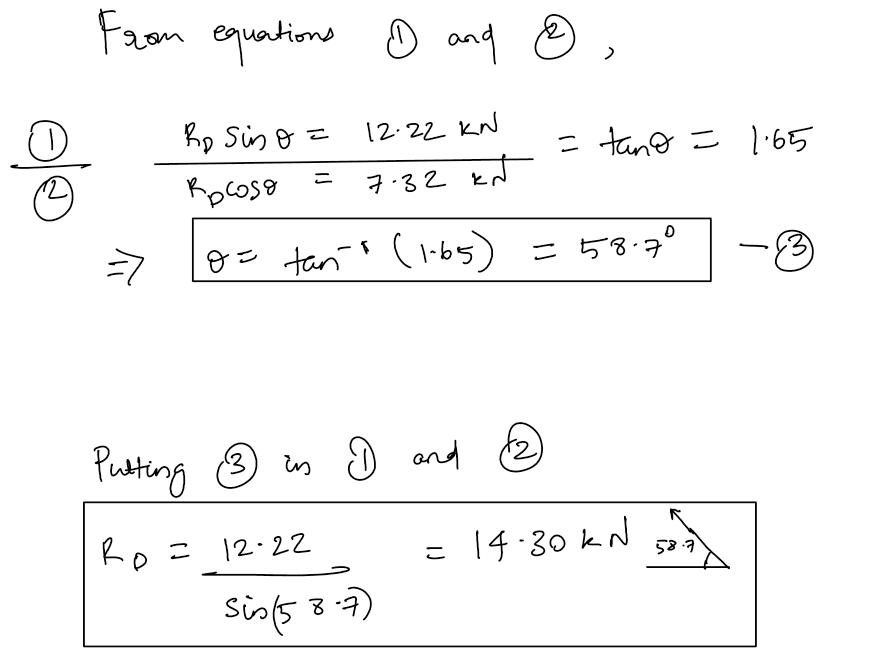
\includegraphics[scale=0.6]{a32.jpg}
	\label{fig: Polygon Law}
\end{figure}

\pagebreak

\section{Graphical Method}

Q1. Determine the magnitude, direction and point of application of resultant from A for the force system shown in Fig. which acts on beam AD.
\begin{figure}[H]
	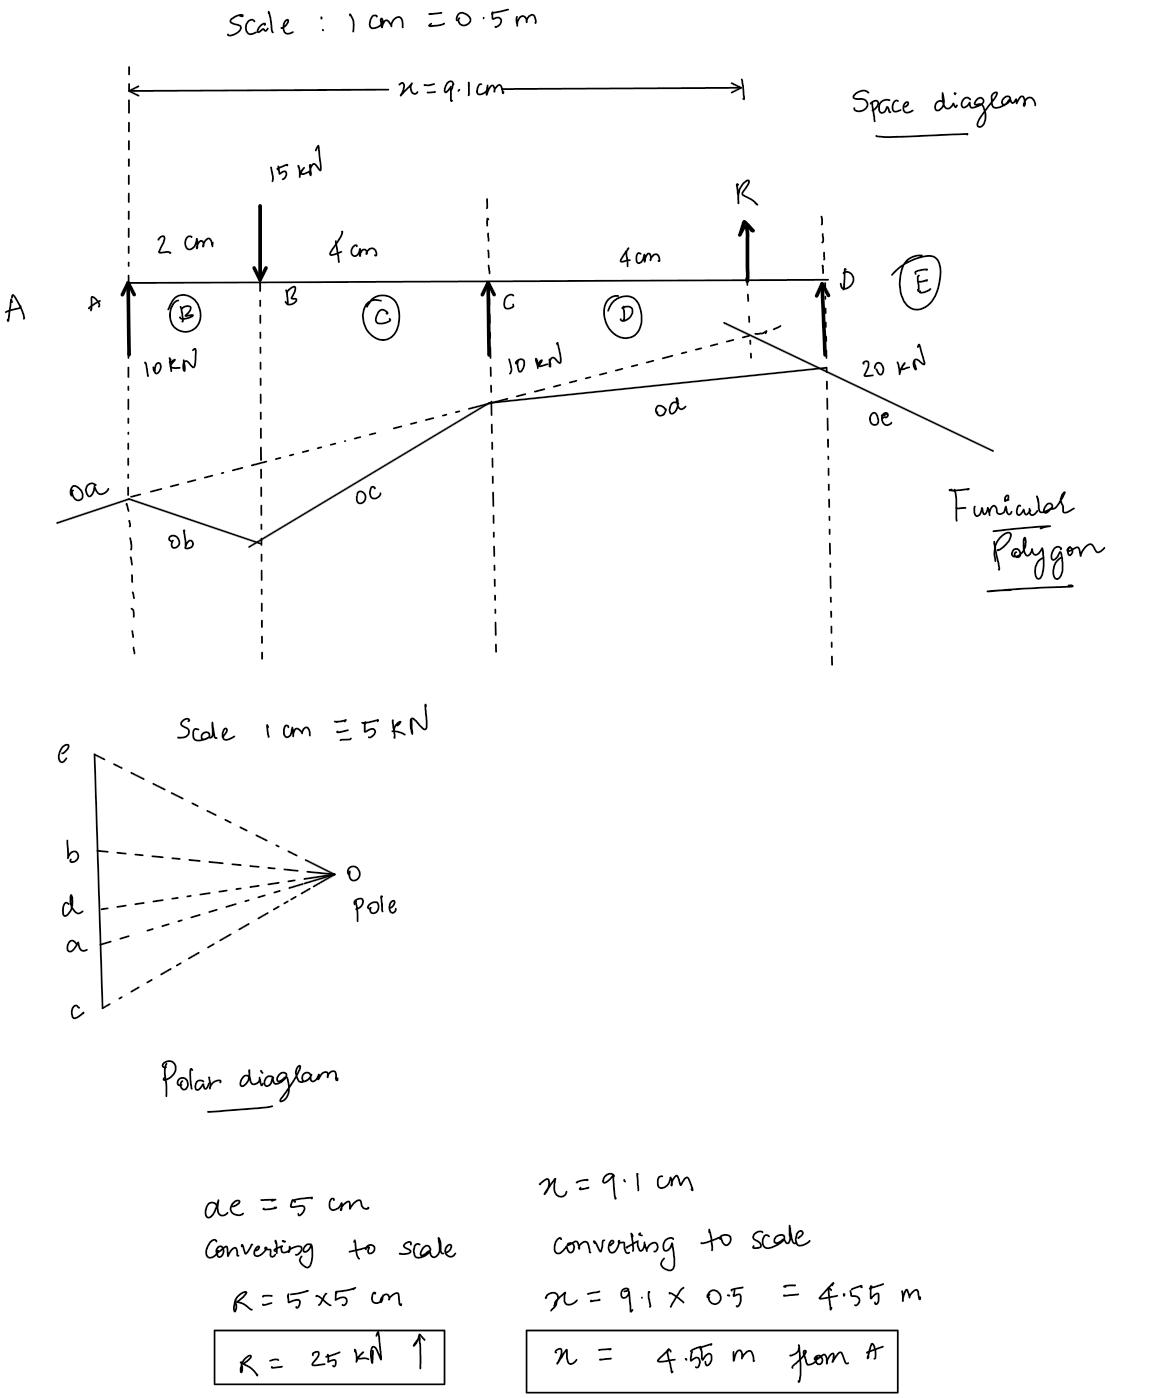
\includegraphics[scale=0.4]{g1.jpg}
	\label{fig: Polygon Law}
\end{figure}


\pagebreak
Q2. Determine the beat reactions for the beam shown in the figure. 
\begin{figure}[H]
	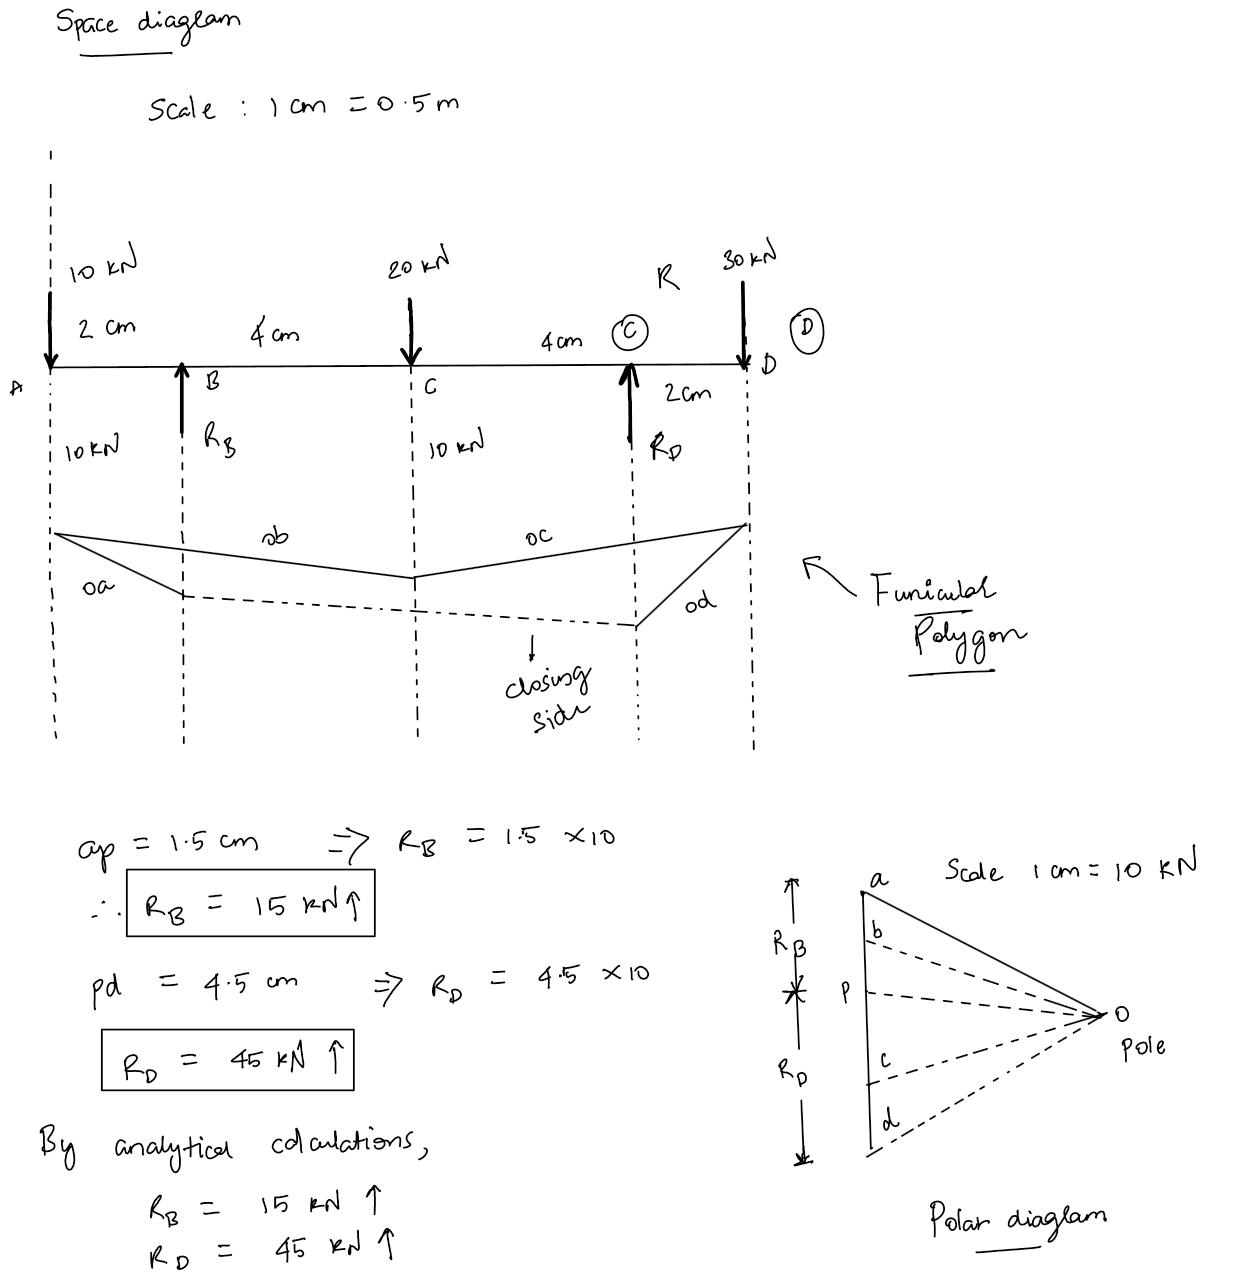
\includegraphics[scale=0.42]{g2.jpg}
	\label{fig: Polygon Law}
\end{figure}

\pagebreak

Q3. Determine support reactions for the beam loaded and supported as shown in the figure.
\begin{figure}[H]
	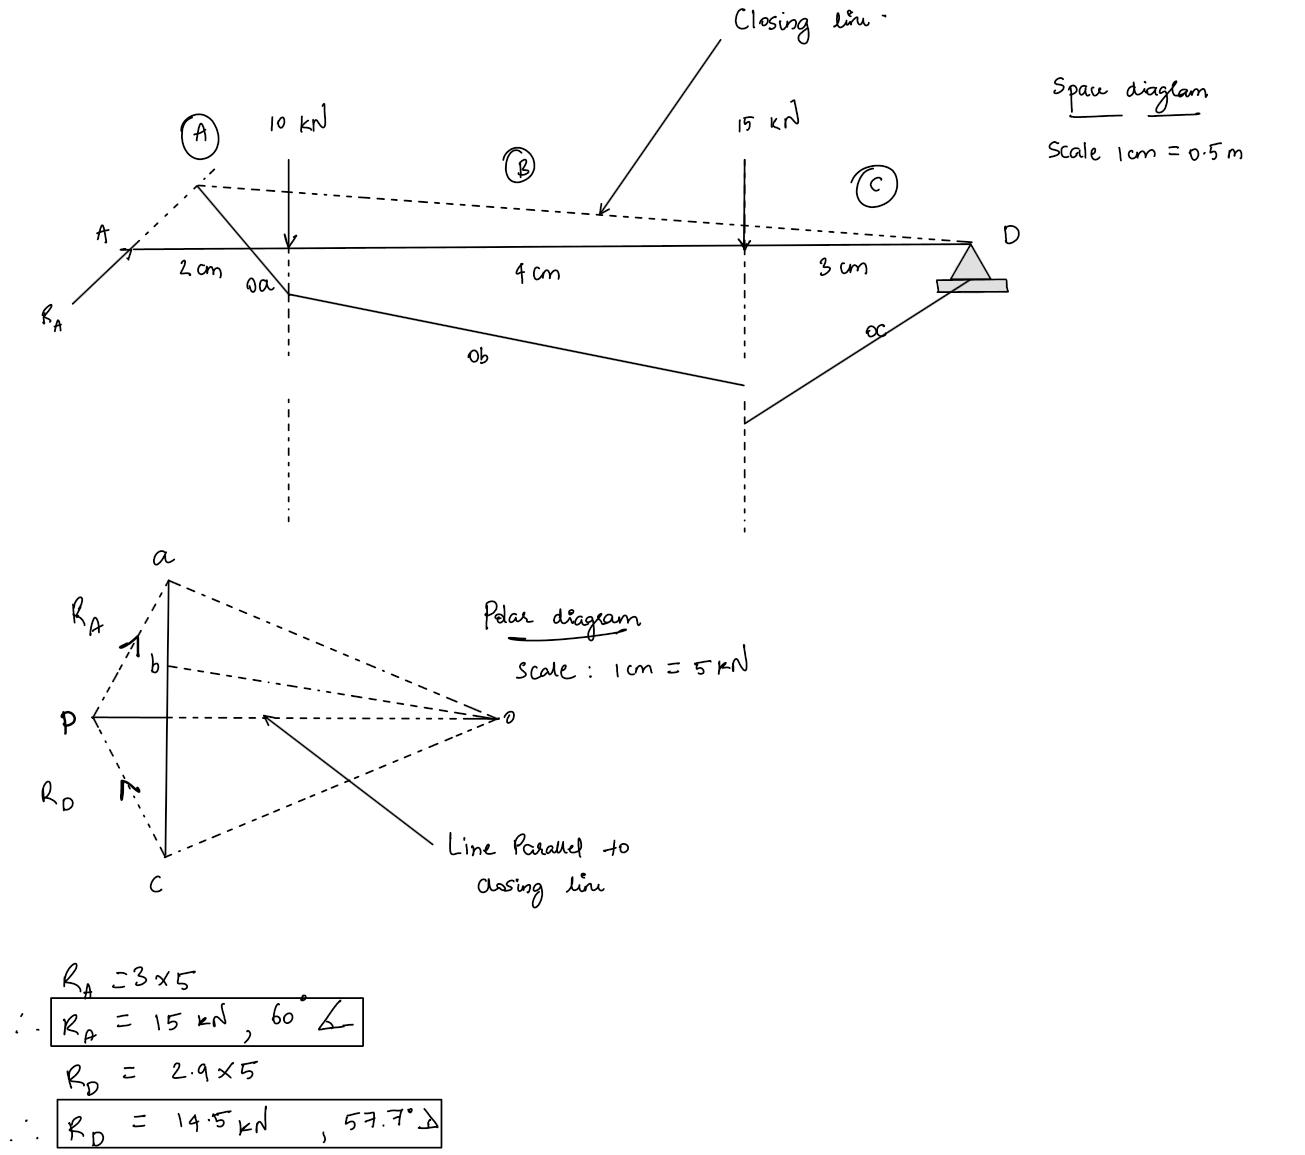
\includegraphics[scale=0.44]{g3.jpg}
	\label{fig: Polygon Law}
\end{figure}

\pagebreak

\section{Results}

\begin{tabular}{|c|c|c|c|}
	\hline
	Question Number & Analytical Solution & Graphical Solution & Percent Error \\
	\hline
	1 	& R = 25 kN  & R = 25 kN & $\eta_R = 0\%$\\
		& $x$ = 4.6 m & $x$ = 4.55 m $\degree$ & $\eta_x = 0.016 \%$\\
	\hline
	2	& $ R_A = 45 kN $ & $ R_A = 45 kN $ & $\eta_{R_A} = 0\%$ \\
		& $ R_B = 15 kN $ & $ R_B = 15 kN $ & $\eta_{R_B} = 0\%$ \\
	\hline
	3	& $ R_A = 14.75 kN $ & $ R_A = 15 kN $ & $\eta_{R_A} = 0.01\%$ \\
		& $ \theta = 58.7\degree $ & $ \theta = 57.7\degree $ & $\eta_\theta = 0.01\%$ \\
	\hline
\end{tabular}


\section{Conclusion}
A set of problems involving Non-concurrent Co-planar Force system were solved using graphical as well as analytical methods. The Percentage error between the two answers was found.
\end{document}